% This document is used for Daya Bay MACRO PMT pressure test report


\documentclass{beamer}
\usepackage{graphicx}
\usepackage{gensymb} %for degree Celsius
\usepackage{mathpazo} % Use the Palatino font
\usepackage{epstopdf} % for including .eps plots

\newcommand{\tabincell}[2]{\begin{tabular}{@{}#1@{}}#2\end{tabular}}

\usepackage{ragged2e}
\justifying

\usepackage{setspace}

\setbeamertemplate{navigation symbols}{}
\setbeamertemplate{footline}[page number]
\setbeamertemplate{caption}[numbered]
\setbeamerfont{caption}{size=\scriptsize}
\usefonttheme{serif} % default family is serif

\usetheme{default}
\begin{document}
\title{Status of MACRO PMT pressure tests at SAB}
\author{Logan Lebanowski, Shih-Kai Lin}
\institute{University of Houston}
\date{2010 December 16}


\begin{frame}{Reverse definition of mean muon energy}
	Given the empirical formula $Y=4.08\bar{E}_{\mu}^{0.78}\equiv \alpha\bar{E}_{\mu}^{\gamma}$, suppose for each single muon this yield is applicable, i.e. replacing $\bar{E}_{\mu}$ with ${E}_{\mu}$, we can calculate the yield as follows:
	\begin{equation*}
	  Y'=\frac{N_n}{N_{\mu}\bar{L}\rho}=\frac{\sum\limits_{i=1}^{N_{\mu}}Y(E_i)\bar{L}\rho }{N_{\mu}\bar{L}\rho}=\frac{\alpha}{N_{\mu}}\sum\limits_{i=1}^{N_{\mu}}E_i^\gamma
	\end{equation*}
	Define
	\begin{equation*}
		\bar{E}'=\left( \frac{Y'}{\alpha} \right) ^{\frac{1}{\gamma}}=\left( \frac{1}{N_{\mu}}\sum\limits_{i=1}^{N_{\mu}}E_i^\gamma \right)^{\frac{1}{\gamma}}
	\end{equation*}
	Note that the mean muon energy corresponds to $\gamma=1$.
\end{frame}


\begin{frame}
	Using the MUSIC energy spectrum as the input, the results of the two mean energies is shown in the table.
	\begin{table}
		\begin{tabular}{|c|c|c|c|}
			\hline
			 & EH1 & EH2 & EH3 \\
			\hline
			$\bar{E}$ (GeV) & 57 & 58 & 137 \\
			$\bar{E}'$ (GeV) & 47 & 48 & 114 \\
			\hline
		\end{tabular}	
	\end{table}
\end{frame}


\begin{frame}{left and right RMS}
	\scriptsize
	If I define
	\begin{equation*}
		left\: RMS=\sqrt{\frac{1}{N_<}\sum\limits_{E_i<\bar{E}}(E_i-\bar{E})^2}
		\;\;\;
		right\: RMS=\sqrt{\frac{1}{N_>}\sum\limits_{E_i>\bar{E}}(E_i-\bar{E})^2}
	\end{equation*}
	then the yield plot will look like
	\begin{center}
		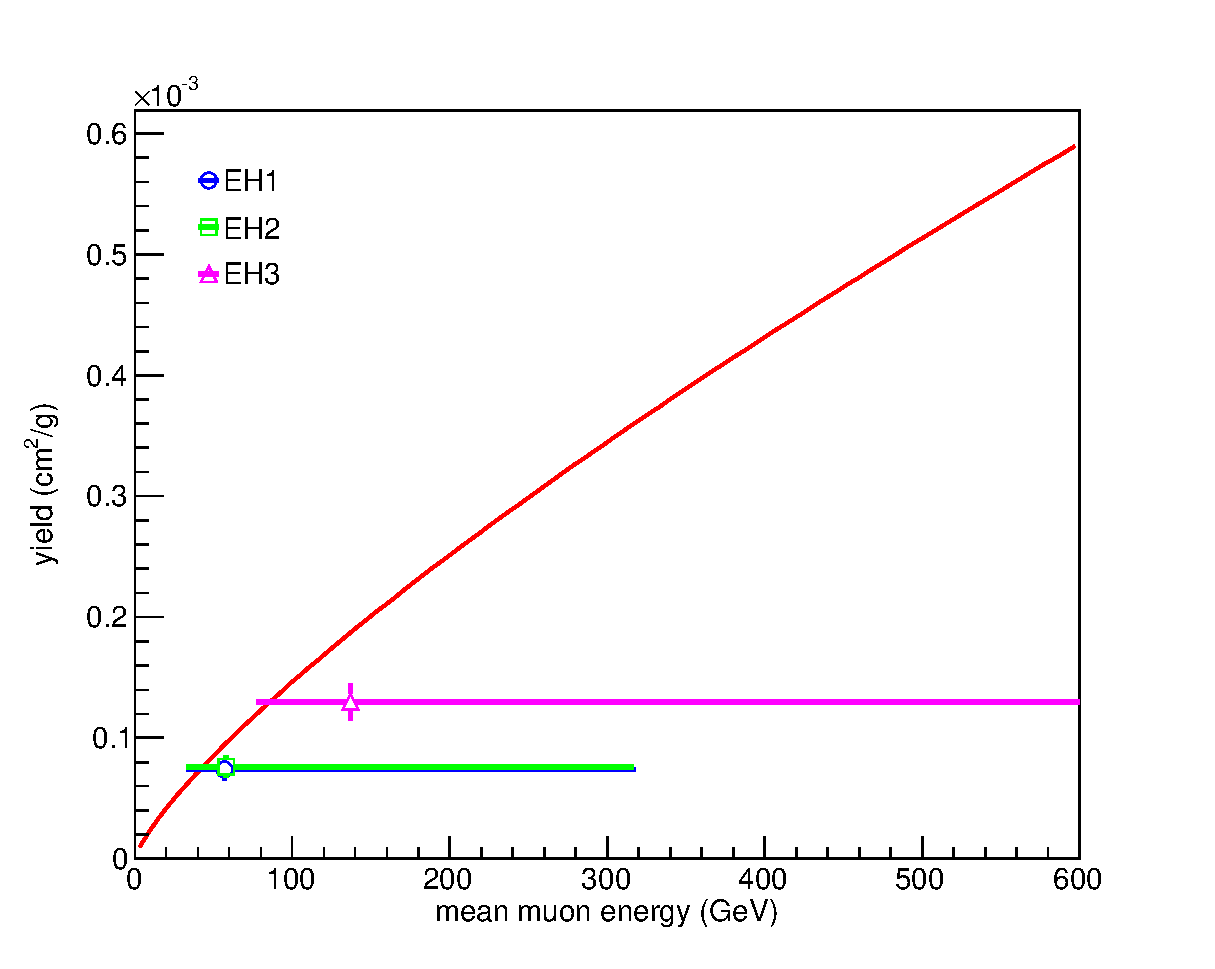
\includegraphics[height=5cm]{LeftRightRMS.eps}
	\end{center}
\end{frame}


\begin{frame}{Comparison with David's \href{http://dayabay.ihep.ac.cn/cgi-bin/DocDB/ShowDocument?docid=8920}{DocDB-8920}}
	\begin{columns}[c]
		\column{.5\textwidth}
			\centering
			Shih-Kai's result
			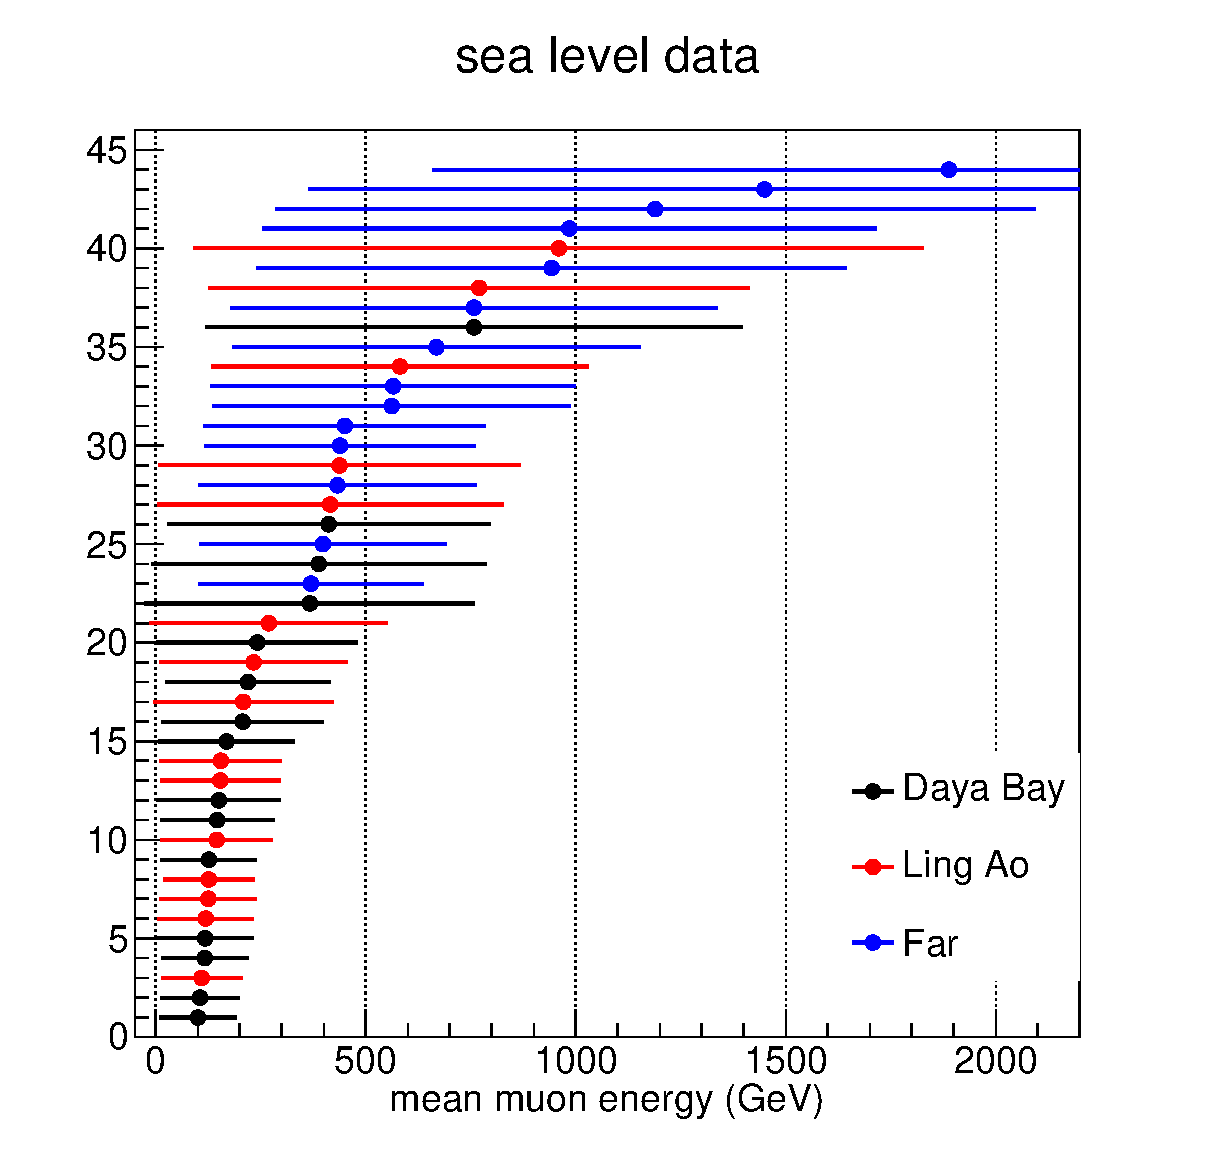
\includegraphics[height=\textwidth]{CompDavid_sea.eps}
		\column{.5\textwidth}
			\centering
			David's result
			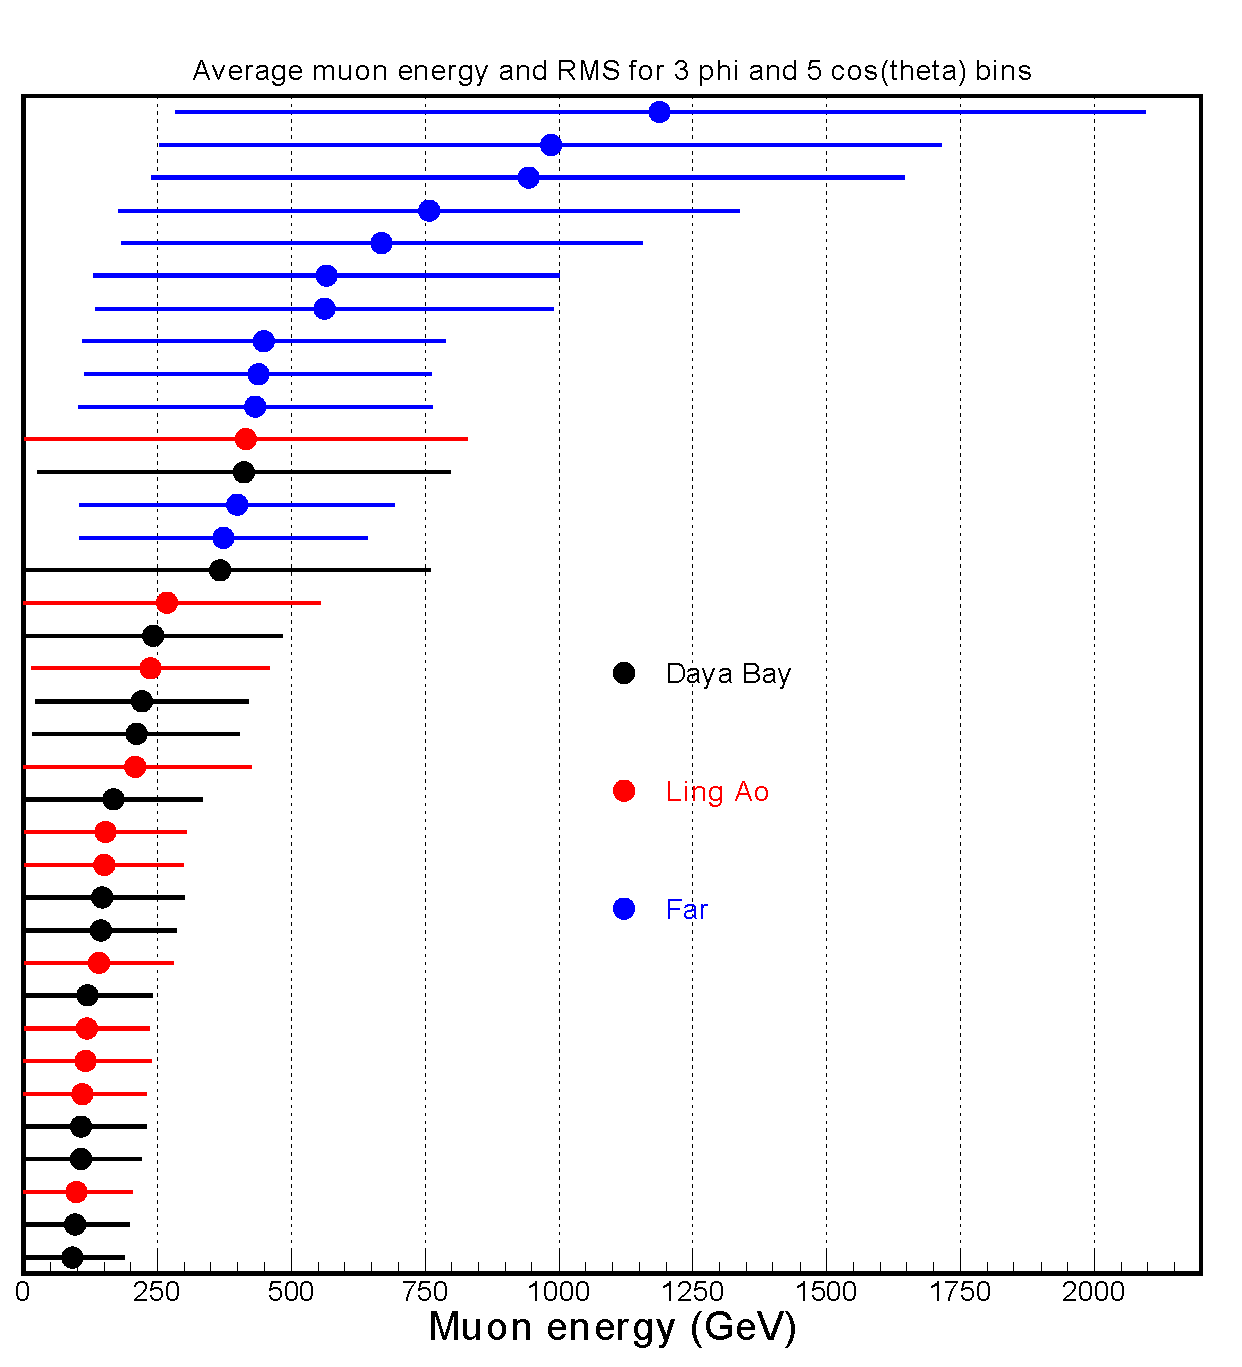
\includegraphics[height=\textwidth]{David_mean_energy.eps}
	\end{columns}
\end{frame}


\begin{frame}{Hall vs. sea level mean muon energy}
	\begin{columns}[c]
		\column{.5\textwidth}
			\centering
			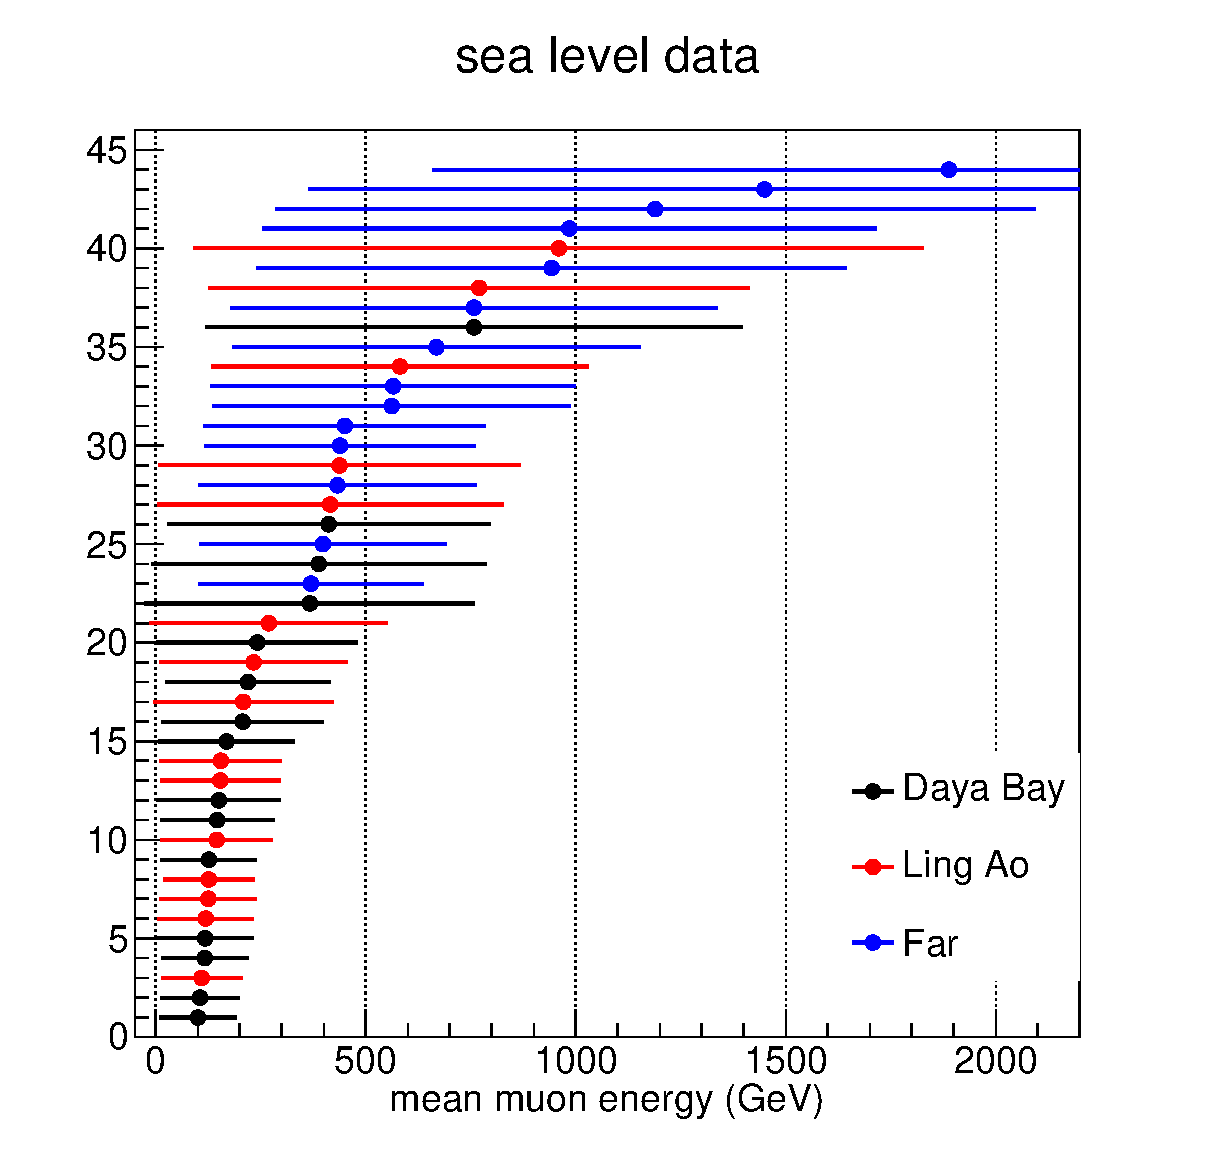
\includegraphics[height=\textwidth]{CompDavid_sea.eps}
		\column{.5\textwidth}
			\centering
			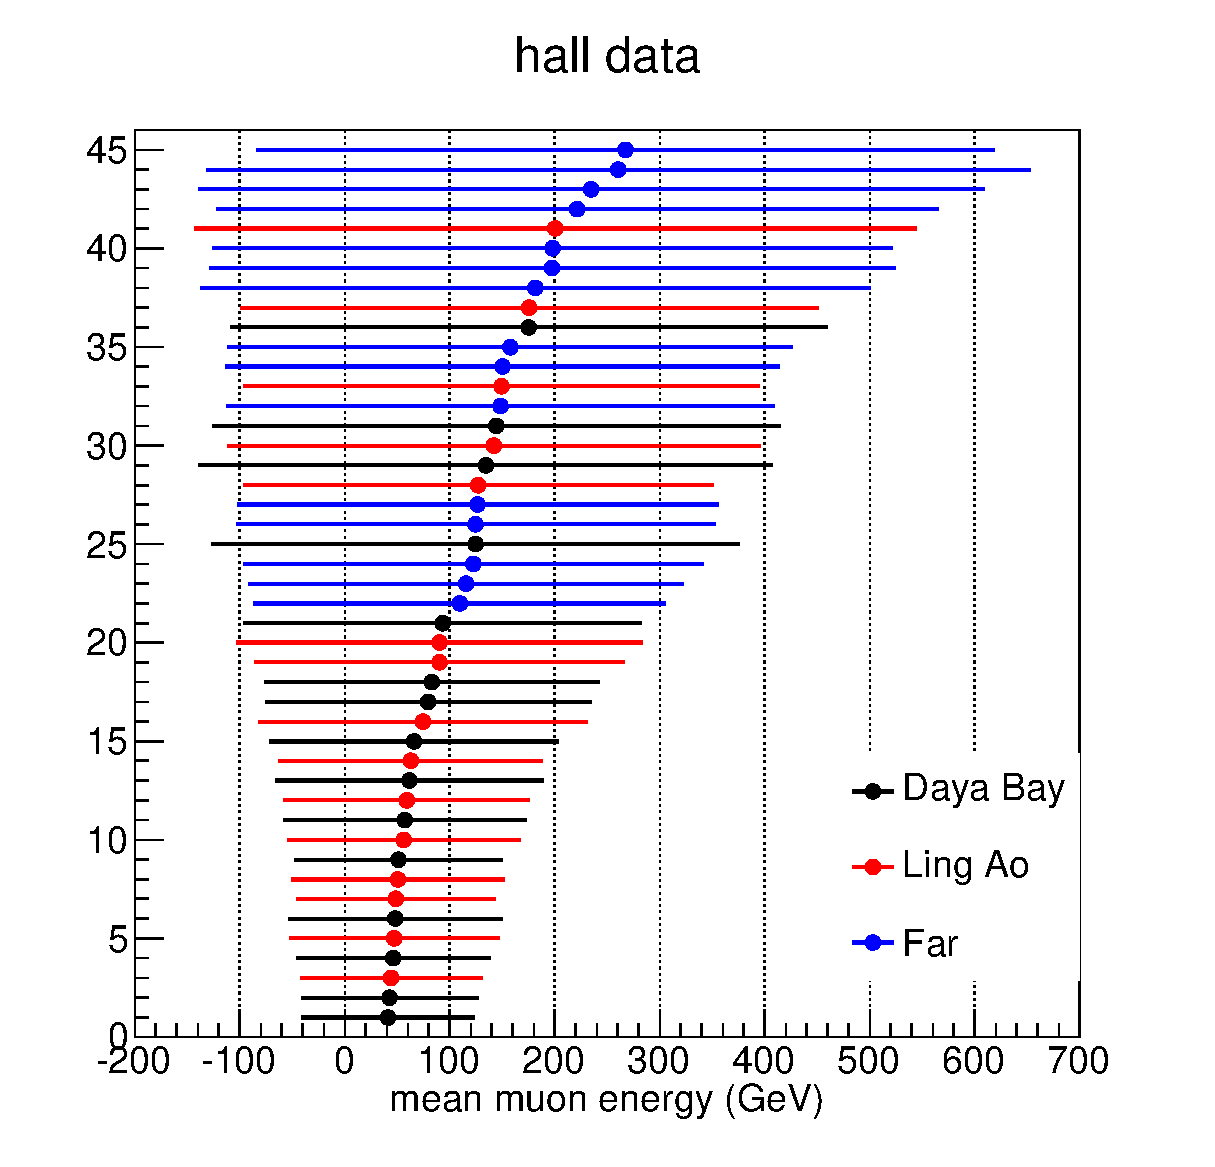
\includegraphics[height=\textwidth]{CompDavid_hall.eps}
	\end{columns}
\end{frame}

\end{document}
